\documentclass{article}
\usepackage{eason}

\usepackage{pdfpages}

\usepackage[a4paper, margin=1in]{geometry}

\usepackage{lipsum}

\newcommand{\DATE}{dummyDate}
\newcommand{\COMMITSHA}{dummySHA}

\title{Lecture 3 -- Euclidean and Coordinate Geometry}
\author{Eason Shao}
\date{v.\DATE.\COMMITSHA}

\begin{document}
\maketitle

\tableofcontents

\section*{More MAT Questions on Trigonometry}

\begin{example}[MAT 2021 Question G]
    Evaluate
    \[
        \sin^2 \pqty{1 \degree} + \sin^2 \pqty{2 \degree} + \sin^2 \pqty{3 \degree} + \cdots + \sin^2 \pqty{89 \degree} + \sin^2 \pqty{90 \degree}.
    \]
\end{example}

\begin{example}[MAT 2011 Question D]
    Find the fraction of the interval \(0 \leq x \leq 2 \pi\) for which
    \[
        \sin x \geq \frac{1}{2} \qor \sin 2x \geq \frac{1}{2}
    \]
    is true.
\end{example}

\section{Geometry in Triangles}
\subsection{Area Formulae, Sine Rule and Cosine Rule}
The very basic one: \(A = \frac{1}{2} ah\).

Area formula in the form of sine:
\[
    A = \frac{1}{2} ab \sin C = \frac{1}{2} ac \sin B = \frac{1}{2} bc \sin A.
\]

Another (potentially) useful one: Heron's formula which states
\[
    A = \sqrt{s \pqty{s - a} \pqty{s - b} \pqty{s - c}}
\]
where \(s = \frac{a + b + c}{2}\).

\begin{problem}
    Prove Heron's formula.
\end{problem}

Sine rule:
\[
    \frac{a}{\sin A} = \frac{b}{\sin B} = \frac{c}{\sin C}.
\]

\textbf{Note that the sine rule always solves for two possible values of an angle, due to the shape of the sine curve.} Sometimes, only one of those angles make sense, while for some other cases, there might be multiple possible triangles (``ambiguity'', see below).

\textbf{When to use sine rule:}
\begin{itemize}
    \item given two angles and one side, find the remaining angle and any other side;
    \item given two sides and one angle but not between them, find another angle.
\end{itemize}

Note: the second case gives rise to ``ambiguity'', see below.

Cosine rule:
\begin{align*}
    a^2 &= b^2 + c^2 - 2bc \cos A \\
    b^2 &= c^2 + a^2 - 2ca \cos B \\
    c^2 &= a^2 + b^2 - 2ab \cos C
\end{align*}

A useful rearrangement of the cosine rule:
\begin{align*}
    \cos A &= \frac{b^2 + c^2 - a^2}{2bc} \\
    \cos B &= \frac{c^2 + a^2 - b^2}{2ca} \\
    \cos C &= \frac{a^2 + b^2 - c^2}{2ab}
\end{align*}

\textbf{When to use cosine rule:}
\begin{itemize}
    \item given three sides, find any angle; (rearrangement)
    \item given two sides and the angle between them, find the third side. (original form)
\end{itemize}

\begin{problem}
    Prove the sine rule and cosine rule.
\end{problem}

\begin{example}[TMUA 2016 P1 Q20]
    The diagram in \autoref{fig:tmua-2016-p1-q20} shows a square-based pyramid with base \(PQRS\) and vertex \(O\). All the edges of the pyramid are of length \(20\) metres.

    Find the shortest distance, in metres, along the outer surface of the pyramid from \(P\) to the midpoint of \(OR\).
\end{example}

\begin{example}[TMUA 2017 P1 Q20]
    The lengths of the sides \(QR\), \(RP\) and \(PQ\) in triangle \(PQR\) are \(a\), \(a + d\) and \(a + 2d\) respectively, where \(a\) and \(d\) are positive and such that \(3d > 2a\). What is the full range, in degrees, of possible values for angle \(PRQ\)?    
\end{example}

\begin{figure}[ht!]
    \centering
    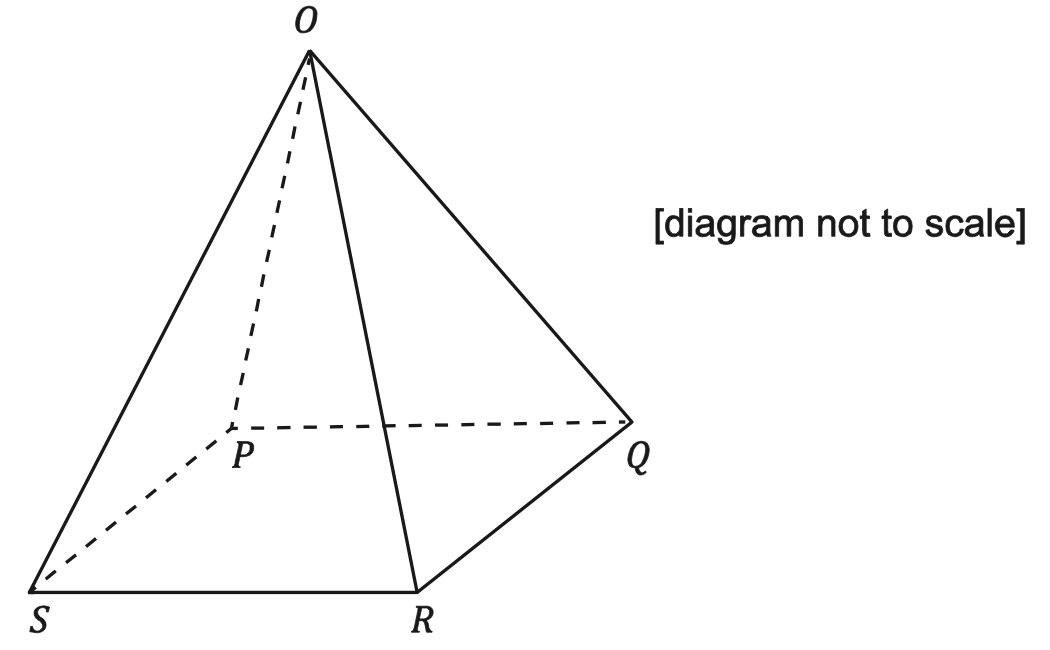
\includegraphics[width=0.7\linewidth]{tmua-2016-p1-q20.png}
    \caption{TMUA 2016 P1 Q20}
    \label{fig:tmua-2016-p1-q20}%
\end{figure}

\subsection{Congruence and Similarity}

\textbf{Congruence} is when two shapes are of the exact same dimensions (i.e. of the exact same shape and size). \textbf{Similarity} is when two shapes are of the same shape (but not necessarily the same size).

Formally speaking, \textbf{congruence} of polygons are when all the edges and the angles correspond (to be equal), while \textbf{similarity} of polygons are when the edges correspond to form a common ratio, and the angles correspond to be equal.

Therefore, congruence is \textbf{strictly a subset} of similarity.

Below, we restrict our view to triangles.

\textbf{Proving congruence from similarity} is by finding any useful information of the size of the triangle, e.g. the length of an edge, or the area of the triangle.

\textbf{Proving similarity} is by:
\begin{itemize}
    \item finding two angles which correspond to be equal (and the third must therefore be);
    \item having all three pairs of edges to be in common ratio;
    \item having two pairs of edges to be in common ration, and the angle in between them to be equal.
\end{itemize}

\textbf{Proving congruence} is by:
\begin{itemize}
    \item \textbf{SSS.} All three sides are equal.
    \item \textbf{SAS.} Two sides and an angle between them.
    \item \textbf{AAS/ASA.} A side and any two angles.
    \item \textbf{RHS.} Right-angled triangle, hypotenuse and any other side (which allows us to find the final side by Pythagorean Theorem).
\end{itemize}

\textbf{SSA} does not necessarily imply congruence -- see ``ambiguity'' case below.

\begin{example}[TMUA 2016 P2 Q9]
    Triangles \(ABC\) and \(XYZ\) have the \textbf{same area}.

    Which of these extra conditions, taken independently, would \textbf{imply} that they are congruent?

    \begin{enumerate}[label=\Roman*]
        \item \(AB = XY\) \textbf{and} \(BC = YZ\)
        \item \(AB = XY\) \textbf{and} \(\angle ABC = \angle XYZ\)
        \item \(\angle ABC = \angle XYZ\) \textbf{and} \(\angle BCA = \angle YZX\)
    \end{enumerate}
\end{example}

\begin{example}[TMUA 2016 P2 Q16]
    In \autoref{fig:tmua-2016-p2-q16}, \(PQRS\) is a trapezium with \(PQ\) parallel to \(SR\). The diagonals of the trapezium meet at \(X\). \(U\) lies on \(SP\) and \(T\) lies on \(RQ\) such that \(UT\) is a line segment through \(X\) parallel to \(PQ\).

    The length of \(PQ\) is \(\SI{12}{\centi\metre}\) and the length of \(SR\) is \(\SI{3}{\centi\metre}\). What, in centimetres, is the length of \(UT\)?
\end{example}

\begin{figure}[ht!]
    \centering
    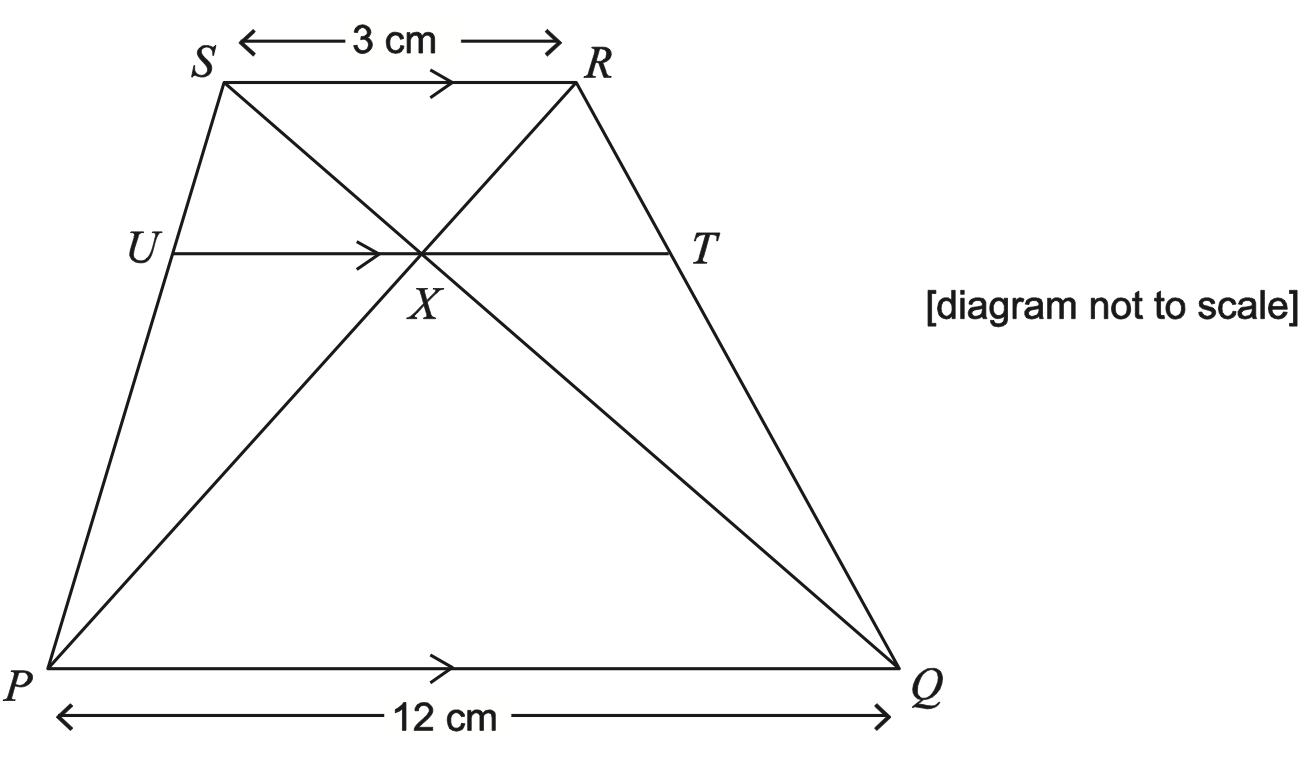
\includegraphics[width=0.8\linewidth]{tmua-2016-p2-q16.png}
    \caption{TMUA 2016 P2 Q16}
    \label{fig:tmua-2016-p2-q16}
\end{figure}

\begin{example}[TMUA 2017 P1 Q20]
    The lengths of the sides \(QR\), \(RP\) and \(PQ\) in triangle \(PQR\) are \(a\), \(a + d\) and \(a + 2d\) respectively. where \(a\) and \(d\) are positive and such that \(3d > 2a\).

    What is the full range, in degrees, of possible values for the angle \(PRQ\)?
\end{example}

\subsection{``Ambiguity'' Case}

When given the length of two sides and an angle that is not between them (the \textbf{SSA}) scenario, there are multiple cases for the dimensions of the triangle. The best way is to draw a diagram, but here is an overview of the possibilities.

Let the edges/angle be \(r, a\) and \(\theta\), in this order. We casework on the value of \(\theta\).

\begin{itemize}
    \item \(\theta < 90\degree\).
    \begin{itemize}
        \item If \(r < a \sin \theta\), the triangle is impossible.
        \item If \(r = a \sin \theta\), the triangle is unique (in which case it is a right-angle triangle).
        \item If \(a \sin \theta < r < a\), there are two possibilities for the triangle, one acute-angled and one obtuse-angled.
        \item If \(r = a\), the triangle is unique (in which case it is an isosceles triangle).
        \item If \(r > a\), the triangle is unique.
    \end{itemize}

    \item \(\theta = 90 \degree\). This reduces to \textbf{RHS}.
    \begin{itemize}
        \item If \(r \leq a\), the triangle is impossible.
        \item If \(r > a\), the triangle is unique.
    \end{itemize}

    \item \(\theta > 90 \degree\).
    \begin{itemize}
        \item If \(r \leq a\), the triangle is impossible.
        \item If \(r > a\), the triangle is unique.
    \end{itemize}
\end{itemize}

\section{Geometry in Circles}
\subsection{Area Formulae}

In the following, \(\theta\) is the angle of the centre, \(r\) is the radius of the circle, and \(d\) is the diameter of the circle.

\textbf{Circumference of a Circle} is (by definition) \(C = 2 \pi r = \pi d\).

\textbf{Arc length} is (by definition) \(l = r \theta\).

\textbf{Area of a Circle} is \(A = \pi r^2 = \flatfrac{\pi d^2}{4}\).

\textbf{Area of a Sector} (pie-shaped, formed by two radii and an arc) is \(A = \frac{1}{2} r^2 \theta\).

\textbf{Area of a Segment} (bow-shaped, formed by a chord and an arc) is \(A = \frac{1}{2} r^2 \pqty{\theta - \sin \theta}\).

\subsection{Circle Properties}

The following list of circle properties is required by the TMUA.

\begin{enumerate}
    \item The perpendicular from the centre to a chord bisects the chord.
    \item The tangent at any point on a circle is perpendicular to the radius at that point.
    \item The angle subtended by an arc at the centre of a circle is twice the angle subtended by the arc at any point on the circumference.
    \item The angle in a semicircle is a right angle.
    \item Angles in the same segment are equal.
    \item The opposite angles in a cyclic quadrilateral add to \(180 \degree\).
    \item The angle between the tangent and chord at the point of contact is equal to the angle in the alternate segment.
\end{enumerate}

\begin{problem}
    Prove the above list of properties.
\end{problem}

\subsection{Relation between Circles}

Let \(d\) be the distance between the centre of the two circles, and \(r_1\) and \(r_2\) be their radii respectively. (We consider the non-degenerate case of \(r_1 \neq r_2\).)

\begin{itemize}
    \item When \(0 \leq d < \abs{r_1 - r_2}\), the smaller circle lies inside the larger circle.
    \item When \(d = \abs{r_1 - r_2}\), the two circles are internally tangent.
    \item When \(\abs{r_1 - r_2} < d < r_1 + r_2\), the two circles intersect at two distinct points.
    \item When \(d = r_1 + r_2\), the two circles are externally tangent.
    \item When \(d > r_1 + r_2\), the two circles are disjoint.
\end{itemize}

\subsection{Miscellaneous}

Two points on a circle split the edge into two parts. The short way around is the \textbf{minor arc} (under \(180 \degree\)), and the long way around is the \textbf{major arc} (over \(180 \degree\)).

\section{Coordinate Geometry}

\subsection{Straight Lines}

There are three ways to represent straight lines:
\begin{enumerate}
    \item \(y - y_1 = m \pqty{x - x_1}\) represents a straight line with gradient \(m\) through the point \(\pqty{x_1, y_1}\);
    \item \(y = mx + b\) represents a straight line with gradient \(m\) and \(y\)-intercept \(b\);
    \item \(ax + by + c = 0\) for \(a, b\) not both zero represents a most general straight line in the plane.
\end{enumerate}

Obviously, the first two forms are equivalent simply by rearranging to get
\[
    b = y_1 - m x_1.
\]

The third option allows us to represent straight lines that \textbf{do not have a gradient}, i.e., vertical lines of the form \(x = m\).

The condition for two lines to be \textbf{parallel} is
\[
    m_1 = m_2,
\]
i.e., having equal gradients.

For them to be \textbf{perpendicular}, we need
\[
    m_1 \times m_2 = -1.
\]

This is especially useful in converting gradient of \textbf{tangents} to gradient of \textbf{normals}.

\begin{example}[TMUA 2017 P1 Q3]
    A line \(l\) has equation \(y = 6 - 2x\). A second line is perpendicular to \(l\) and passes through the point \(\pqty{-6, 0}\).

    Find the area of the region enclosed by the two lines and the \(x\)-axis.
\end{example}

In the form of \(ax + by + c = 0\), it is useful to convert those back to the gradient-intercept form. Special cases that cannot be converted (i.e. the vertical line) can simply be dealt with separately.

Although not required, the following results could be really handy.

Two lines of the form \(a_1 x + b_1 y + c_1 = 0\) and \(a_2 x + b_2 y + c_2 = 0\) are parallel, if and only if the vectors
\[
    \pmqty{a_1 \\ b_1} \qand \pmqty{a_2 \\ b_2}
\]
are parallel (i.e., one is a multiple of another).

The distance from a point \(\pqty{x, y}\) to the line \(ax + by + c = 0\) is
\[
    \frac{\abs{a x + b y + c}}{\sqrt{a^2 + b^2}}
\]
and the distance between two parallel lines \(ax + by + c_1 = 0\) and \(ax + by + c_2 = 0\) is
\[
    \frac{\abs{c_1 - c_2}}{\sqrt{a^2 + b^2}}.
\]

\begin{problem}
    Prove the above formulae.
\end{problem}

\begin{example}[TMUA 2017 P2 Q2]
    \(PQRS\) is a rectangle. The coordinates of \(P\) and \(Q\) are \(\pqty{0, 6}\) and \(\pqty{1, 8}\) respectively. The perpendicular to \(PQ\) at \(Q\) meets the \(x\)-axis at \(R\). What is the area of \(PQRS\)?
\end{example}

\subsection{Circles}

The equation of a circle with \textbf{centre} \(\pqty{a, b}\) and \textbf{radius} \(r\) is
\[
    \pqty{x - a}^2 + \pqty{y - b}^2 = r^2.
\]

\begin{example}[TMUA 2016 P1 Q9]
    The line segment joining the points \(\pqty{3, 3}\) and \(\pqty{7, 5}\) is a diameter of a circle.

    The circle is translated by \(3\) units in the negative \(x\)-direction, then reflected in the \(x\)-axis, and then enlarged by a scale factor of \(4\) about the centre of the resulting circle.

    Find the equation of the final circle.
\end{example}

Expanding the brackets completely, the equation of a circle may also take the form of
\[
    x^2 + y^2 + cx + dy + e = 0.
\]

Completing the square gives us
\[
    \pqty{x + \frac{c}{2}}^2 + \pqty{y + \frac{d}{2}}^2 = \frac{c^2 + d^2}{4} - e
\]
and we indeed need the radius squared to be positive, so we need
\[
    4e < c^2 + d^2.
\]

When solving for the equation of a tangent, it is often helpful to use the fact that tangents and circles only intersect at one point, rather than that they ``share a gradient'' (i.e. solving by differentiating). (This is also useful for solving when a line intersects with a quadratic exactly once.)

\begin{example}
    Find the values of \(c\) for which \(y = 2x + c\) is tangent to the circle with equation \(\pqty{x - 3}^2 + \pqty{y - 2}^2 = 9\).
\end{example}

\begin{example}
    Find the closest distance between the line \(y = x + 11\) and the circle \(\pqty{x + 2}^2 + \pqty{y - 3}^2 = 9\).
\end{example}

\begin{example}[TMUA 2017 P1 Q6]
    A tangent to the circle \(x^2 + y^2 = 144\) passes through the point \(\pqty{20, 0}\) and crosses the positive \(y\) axis.

    What is the value of \(y\) at the point where the tangent meets the \(y\)-axis?
\end{example}

\begin{example}[TMUA 2017 P1 Q9]
    A circle has equation \(x^2 + y^2 - 18 x - 22 y + 178 = 0\). A regular hexagon is drawn inside this circle so that the vertices of the hexagon touch the circle. What is the area of the hexagon?
\end{example}

\begin{example}[MAT 2009 Question B]
    The point on the circle
    \[
        x^2 + y^2 + 6x + 8y = 75
    \]
    which is closest to the origin, is at what distance from the origin?
\end{example}

\begin{example}[MAT 2011 Question F]
    Given \(\theta\) in the range \(0 \leq \theta < \pi\), the equation
    \[
        x^2 + y^2 + 4x \cos \theta + 8y \sin \theta + 10 = 0
    \]
    represents a circle for which range of \(\theta\)?
\end{example}

\begin{example}[MAT 2016 Question C]
    The origin lies inside the circle with equation
    \[
        x^2 + ax + y^2 + by = c
    \]
    precisely when
    \begin{enumerate}[label=(\alph*)]
        \item \(c > 0\)
        \item \(a^2 + b^2 > c\)
        \item \(a^2 + b^2 < c\)
        \item \(a^2 + b^2 > 4c\)
        \item \(a^2 + b^2 < 4c\)
    \end{enumerate}
\end{example}

\subsection{Polygons}

The sum of \textbf{external} angles of polygons is always \(360 \degree\).

The sum of \textbf{internal} angles of a \(n\)-sided polygon is \(\pqty{n - 2} \cdot 180 \degree\), which means the internal angle of a regular \(n\)-sided polygon (whose sides and angles are all equal) is \(\frac{n - 2}{n} \cdot 180 \degree\).

\begin{example}[TMUA 2016 P2 Q20]
    Each interior angle of a regular polygon with \(n\) sides is \(\flatfrac{3}{4}\) of each interior angle of a second regular polygon with \(m\) sides. How many pairs of positive integers \(n\) and \(m\) are there for which this statement is true?
\end{example}

\section{Geometry in Three Dimensions}
\subsection{Geometric Shapes}

A \textbf{sphere} has surface area \(4 \pi r^2\) and volume \(\frac{4}{3} \pi r^3\). (You cannot expand the surface of a sphere, since it is curved.)

A \textbf{cylinder} has surface area \(2 \pi r^2 + 2 \pi r h\) and volume \(\pi r^2 h\). It expands to two circles and a rectangle.

A \textbf{cone} has surface area \(\pi r^2 + \pi r \sqrt{r^2 + h^2}\) and volume \(\frac{1}{3} \pi r^2 h\). It expands to a sector and a circle.

A \textbf{prism} is a shape with a polygon as its base and extends straight up to a certain height. Its volume is given by base area multiplied by height, and its surface area is given by the circumference of the polygon multiplied by the height, plus double the area of the polygon.

A \textbf{pyramid} is a shape with a polygon as its base, but extends linearly up to converge at a single point. Its volume is one-third the volume of a corresponding prism.

\begin{example}[TMUA 2016 P1 Q12]
    A right circular cylinder is contained within a sphere of radius \(\SI{5}{\centi\metre}\) in such a way that the whole of the circumferences of both ends of the cylinder are in contact with the sphere.

    The diagram in \autoref{fig:tmua-2016-p1-q12} shows a planar cross section through the centre of the sphere and the cylinder.

    Find, in cubic centimetres, the maximum possible volume of the cylinder.
\end{example}

\begin{figure}[ht!]
    \centering
    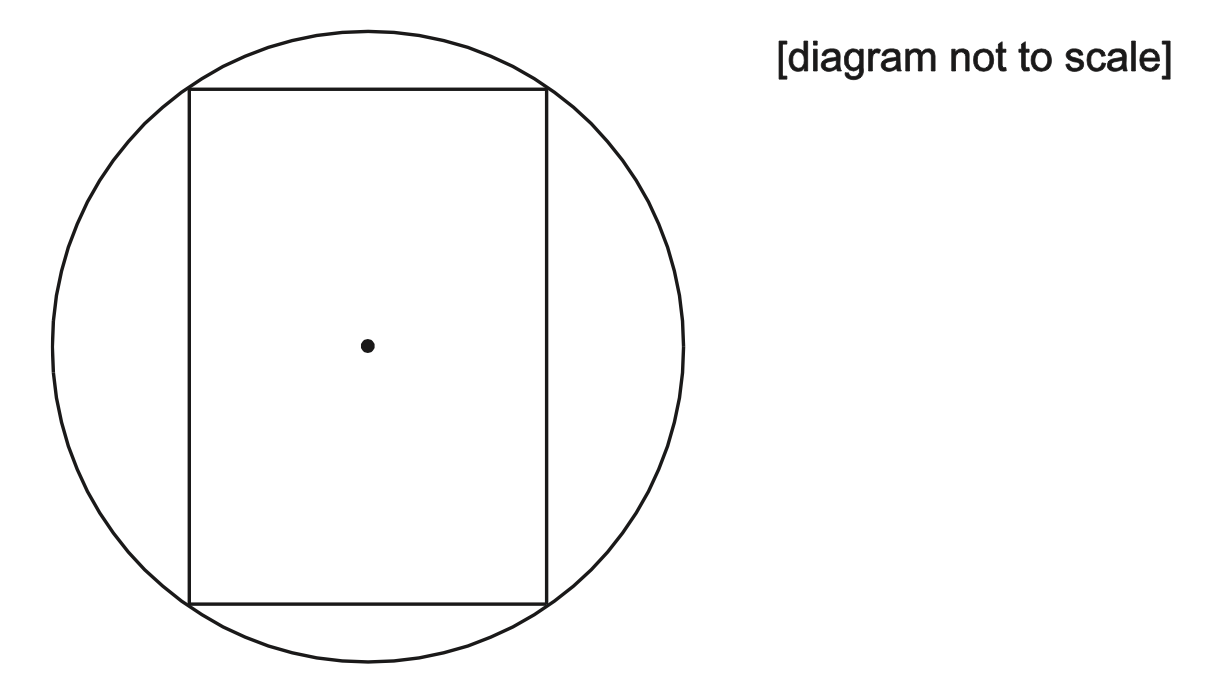
\includegraphics[width=0.6\linewidth]{tmua-2016-p1-q12.png}
    \caption{TMUA 2016 P1 Q12}
    \label{fig:tmua-2016-p1-q12}
\end{figure}

\subsection{Plans and Elevation}

I would recommend watching \href{https://www.bilibili.com/video/BV1tQ4y1q7Sw/?share_source=copy_web}{this video} on counting cubes. Always label the height on the plan view.

\begin{example}[TMUA 2016 P1 Q19]
    Some identical unit cubes are used to construct a three-dimensional object by gluing them together face to face.

    Sketches of this object are made by looking at it from the right-hand side, form the front and from above. These sketches are called the side elevation, the front elevation, and the plan view respectively.

    How many cubes were used to construct the object?
\end{example}

\begin{figure}[ht!]
    \centering
    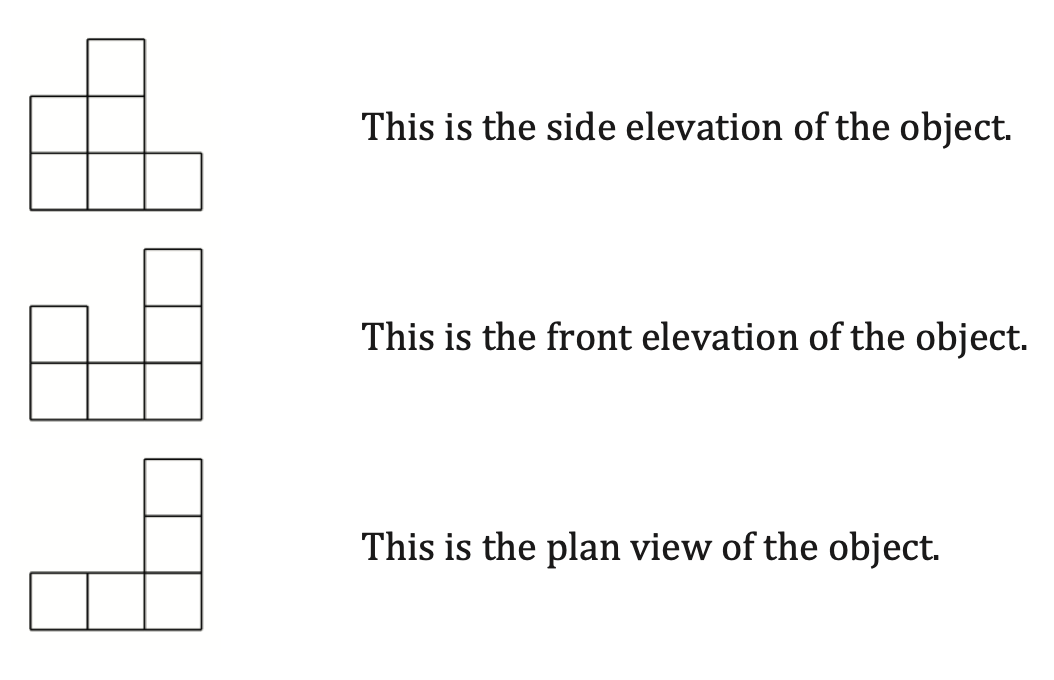
\includegraphics[width=0.6\linewidth]{tmua-2016-p2-q19.png}
    \caption{TMUA 2016 P2 Q19}
    \label{fig:tmua-2016-p2-q19}
\end{figure}

\end{document}